\documentclass[runningheads,a4paper]{llncs}
\usepackage[utf8]{inputenc}
\usepackage[english]{babel}
\usepackage{pdfpages, titling}
\usepackage{array, float}
\usepackage{booktabs}
\usepackage{cite, tablefootnote}
\usepackage{graphicx, caption, subfigure, wrapfig}
\usepackage{listings}
\usepackage{geometry}
\usepackage{color}
\usepackage{mathtools, braket}
\usepackage{amssymb}
\usepackage[nottoc]{tocbibind} % references in the toc
\usepackage{etoolbox}

\geometry{
	includeheadfoot,
    margin=2.54cm
}

\usepackage{footnote}
\makesavenoteenv{tabular}
\makesavenoteenv{table}

\usepackage{textcomp}
\usepackage{minted}
\usepackage[hidelinks]{hyperref}
\graphicspath{{Pictures/}} % Specifies the directory where pictures are stored/

\newcommand{\vect}[1]{\boldsymbol{#1}}
\renewcommand{\subtitle}[1]{
  \posttitle{
    \par\end{center}
    \begin{center}\large#1\end{center}
    \vskip0.5em}
}

\author{Jaro Camphuijsen (jcn690), Rahiel Kasim (rkm700), Jan Westerdiep (jwp800)}
\date{\today}
\title{Data Mining Techniques}
\subtitle{Databeestjes}
\patchcmd{\thebibliography}{\chapter*}{\section*}{}{}
\begin{document}
\maketitle

\section{Exploring a small data set}
\begin{wraptable}{r}{.35 \linewidth}
\vspace{-50pt}
  \begin{tabular}{lll}\\\toprule
   Col &Question & Type\\\midrule
  	1& Study programme &enum\\ 
  	2-5&Courses ($4 \times$) &bool \\ 
  6 &Gender &enum \\
  7 &Chocolate makes you... &enum \\
  8 &Birthday &date \\
  9 &Neighbour count &int \\
  10 &Stand up? &bool \\
  11 &Stress level &float \\
  12 &Money question &float\\
  13 &Random number &float \\
  14 &Bedtime &time \\
  15-16 &Good day? &string\\\bottomrule
  \end{tabular}
  \caption{The different attributes for the given data set.}
  \label{tbl:attribs}
  \vspace{-50pt}
\end{wraptable}

For this task, we decided to use Python with sklearn, as we are proficient in the language and heard good things about the package.  The data set is quite nice; we have little missing data values, and most of the attributes are easily parsed.  In total, we have 129 data points with 16 attributes, distributed over 13 questions; see Table~\ref{tbl:attribs}.

What immediately jumps out is the fact that each binary question has its own representation, so we will have to parse this.  Moreover, we see that only two people stood up; we will refrain from using attribute 10.  Lastly, a few of the enumerative questions had nonlegal answers which we will have to filter out.  This results in a few missing data points.

In a recent lecture,\cite{lecture2DataMining} a very nice broad exploratory analysis was made; instead of repeating these results, we chose to look at some specific interesting points.

\subsection{Study programmes}

It seems there are only a few different study programmes, or combinations of those, in which students are enrolled. See the left of Figure~\ref{fig:studies}.  The majority of the students is enrolled in the programmes Artificial Intelligence, Business Analytics, and Computational Science; this is explained by the fact that Data Mining is an elective course for each of these programmes.  

\begin{figure}[t]
\centering
  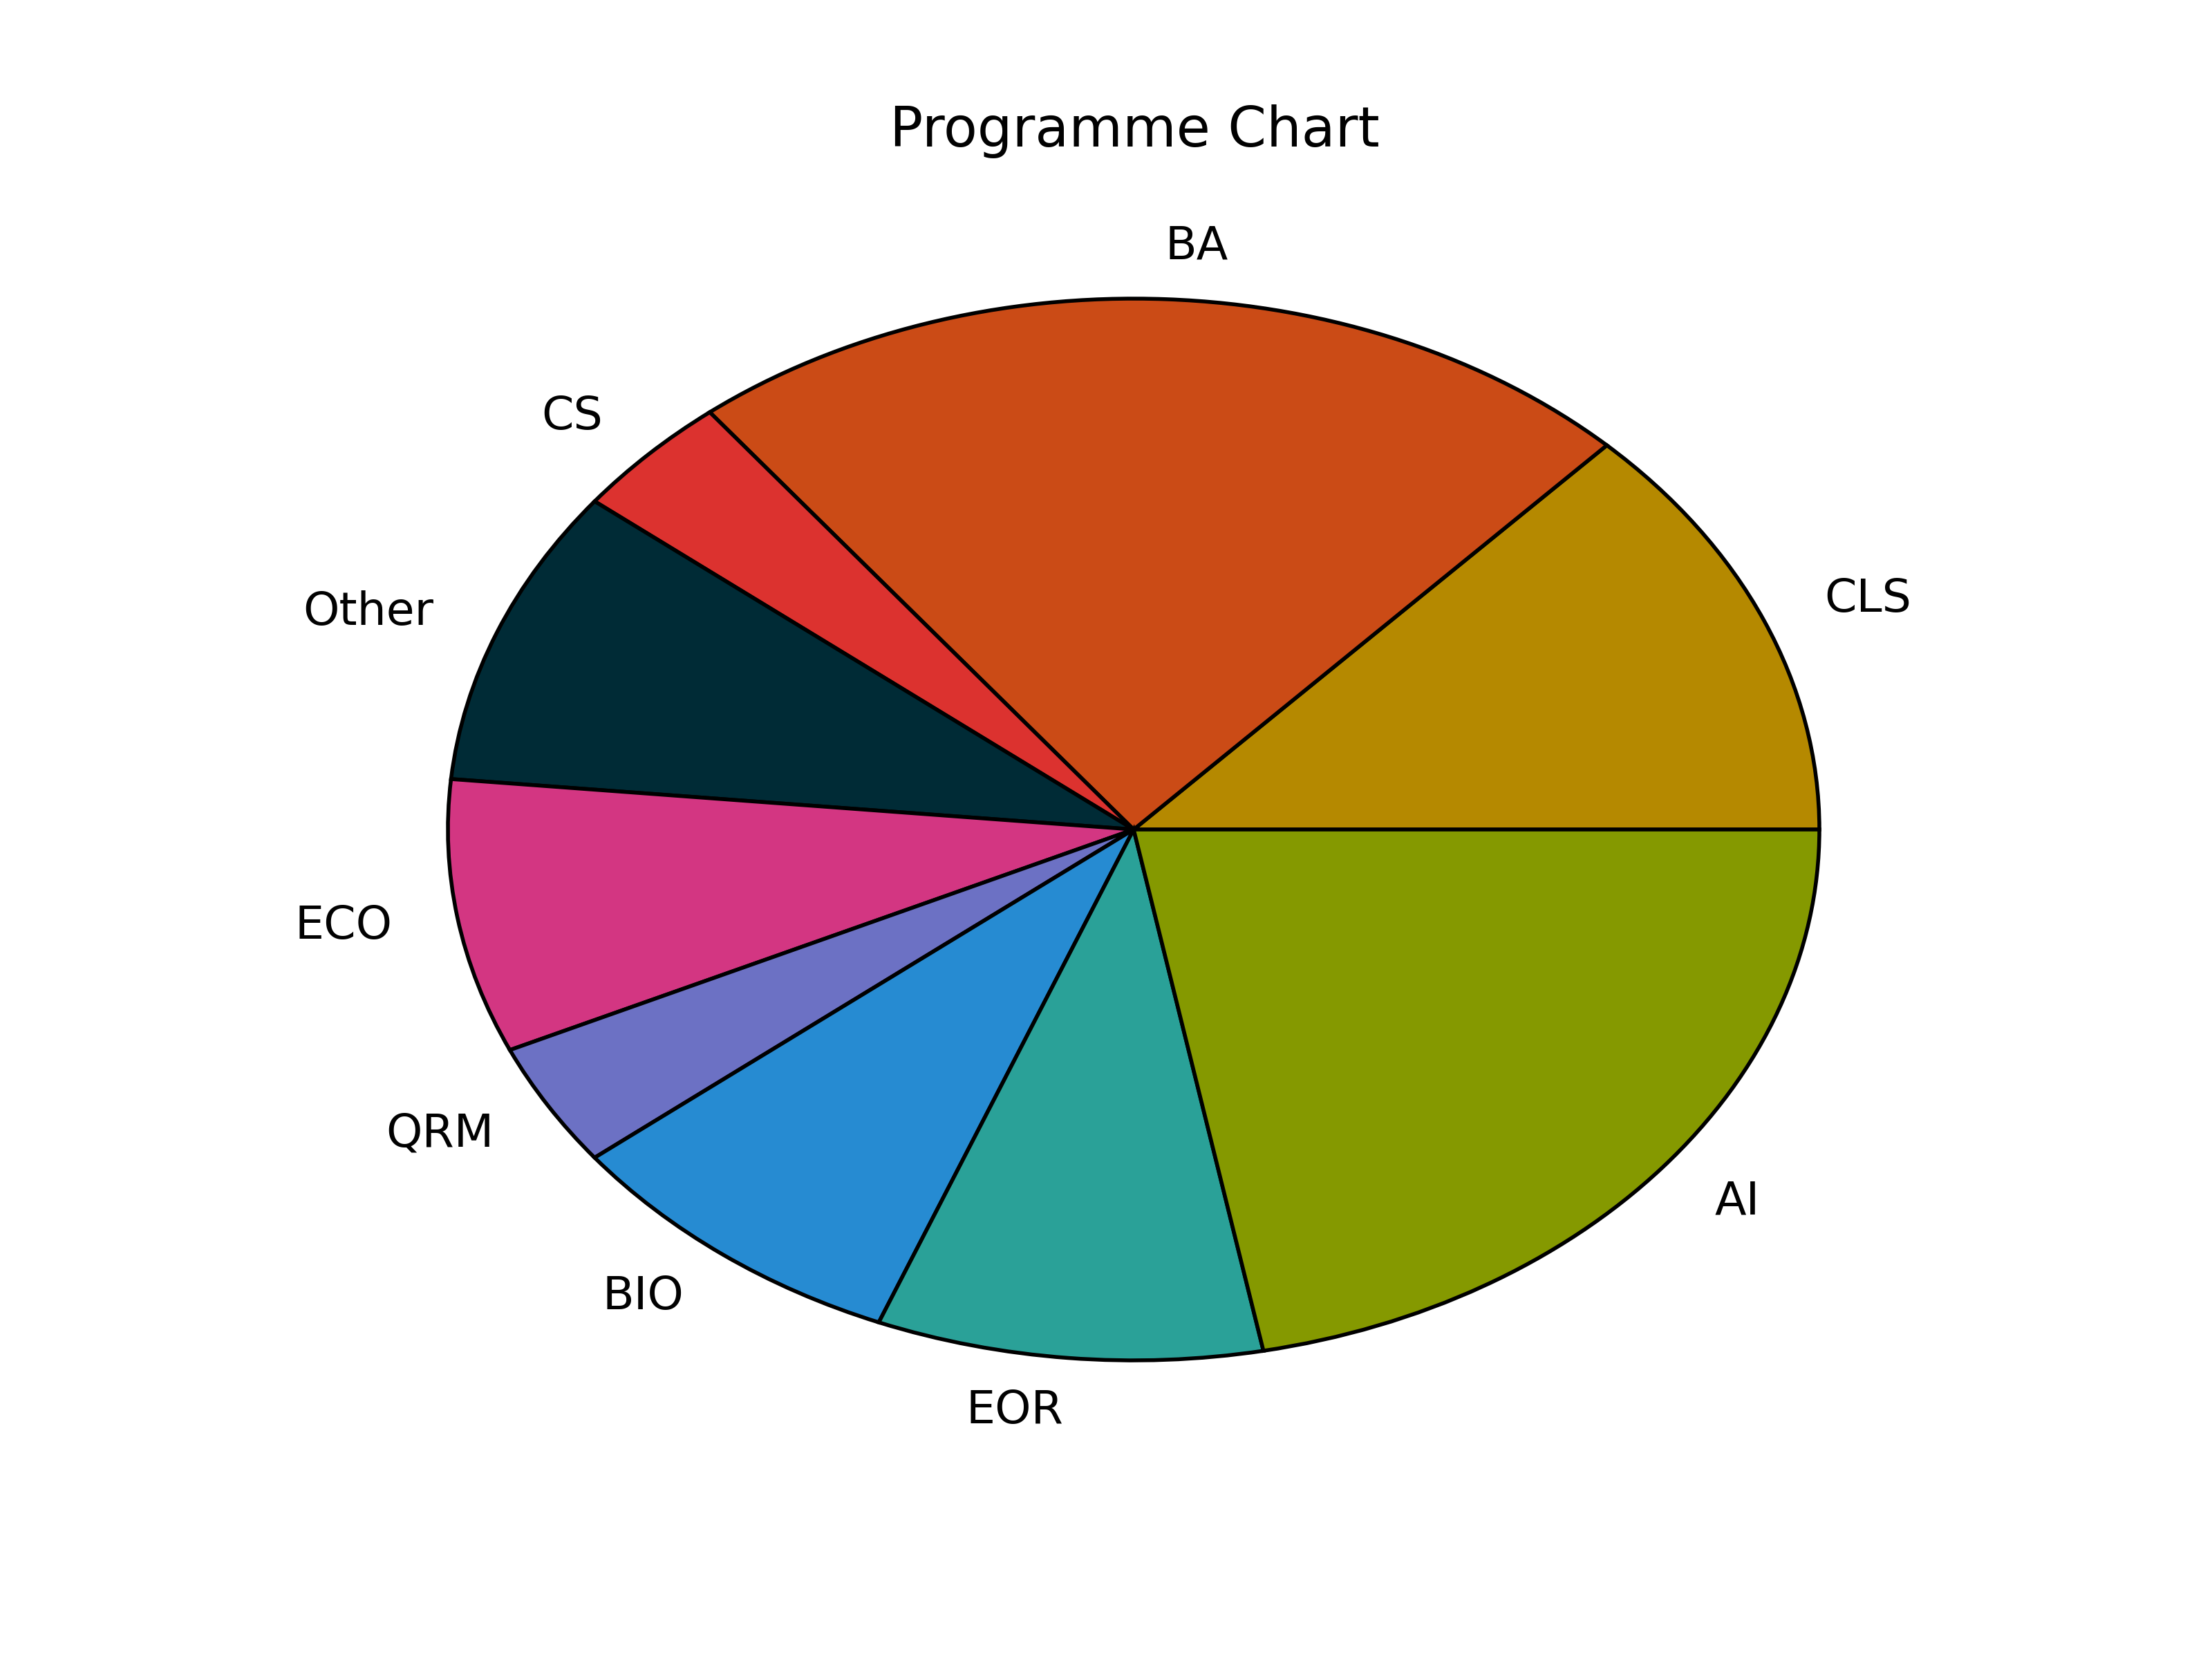
\includegraphics[width=0.49\textwidth]{programme_pie}
  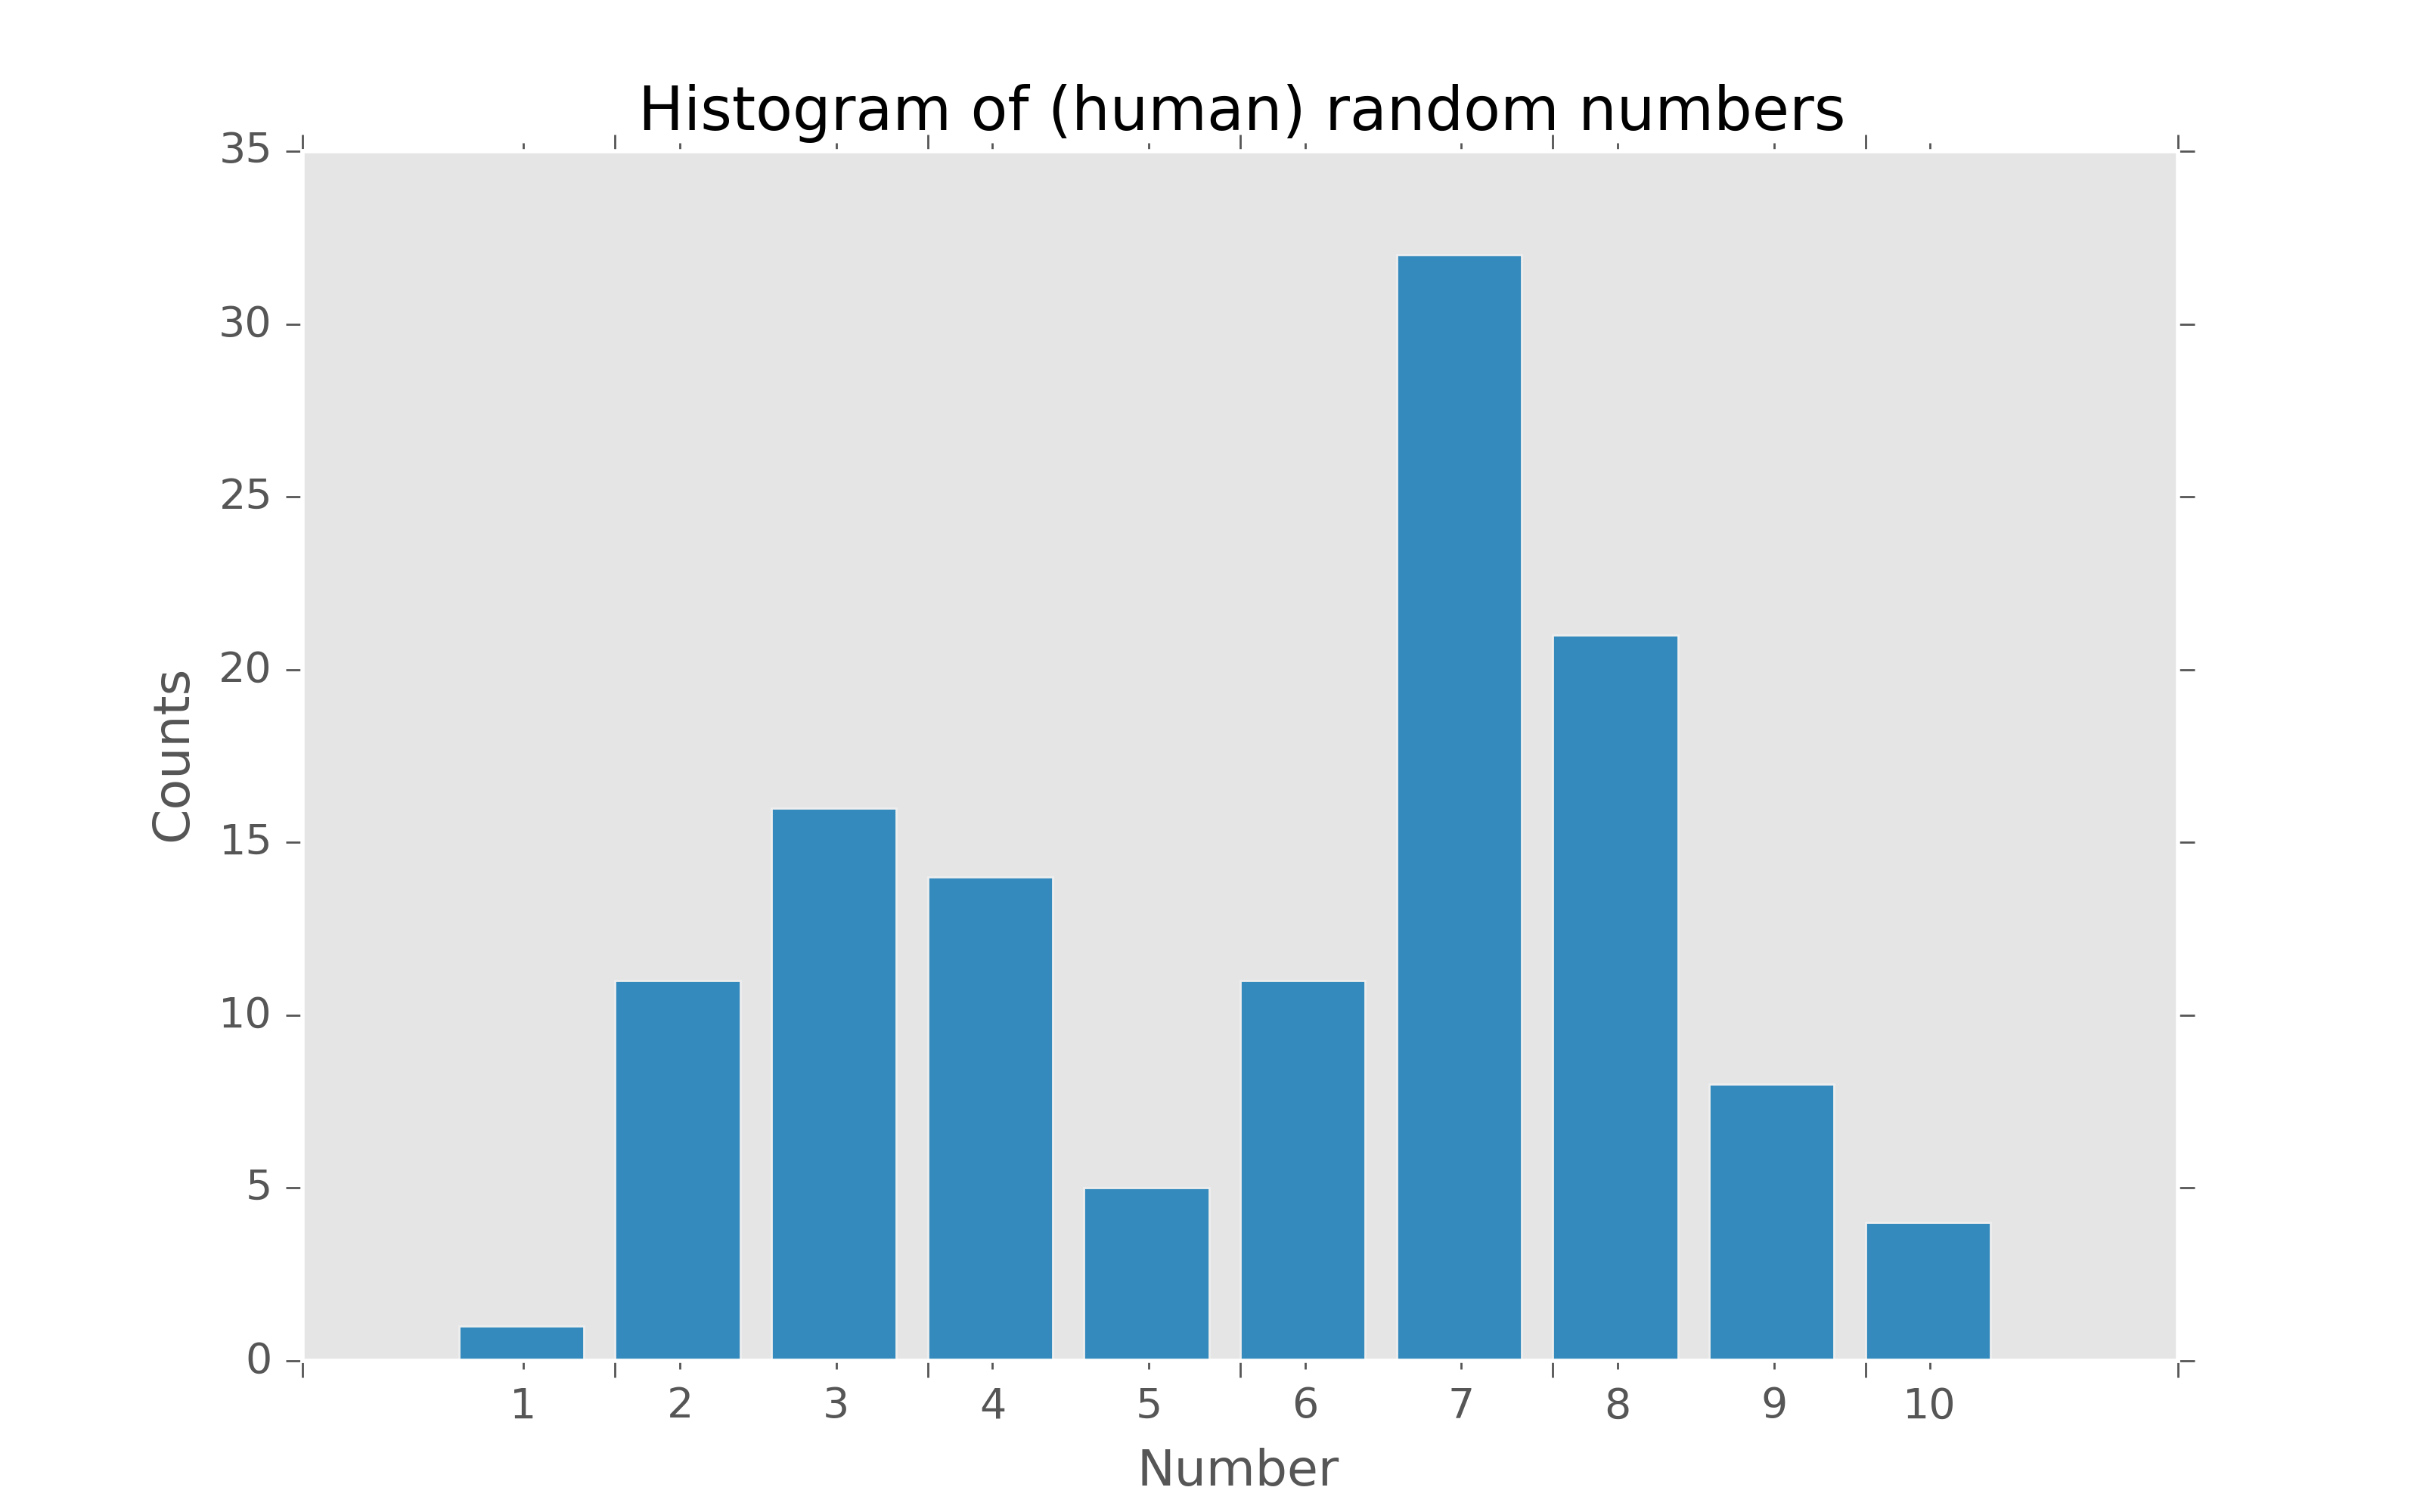
\includegraphics[width=0.49\textwidth]{random_human_nums}
  \caption{Left: The distribution of different study programmes of the students enrolled in this course. Right: The distribution of random numbers generated by the students enrolled in this course. }
  \label{fig:studies}
\end{figure}

\subsection{Birthday problem}
Consider the following: in a group of $n$ people, what is the probability that two people share the same birthday? The exact answer\cite{wiki:birthday}	 to this is
\[
 p(n) = 1 - \frac{365!}{365^n (365-n)!}.
\]
In our case, this probability amounts to $\approx 1 - 6 \cdot 10^{-12}$; looking at the data set, we see that indeed there are birthday collisions. In fact, we have four collisions on February 14! The probability of this is much harder to compute explicitly \cite{birthday}; for $n \to \infty$, a good approximation to this turns out to be
\[
 p(n, m) = 1 - \exp\left(-{n \choose m} / 365^{m-1}\right) \implies p(128, 4) \approx 19.7\%,
\]
which makes the quadruple occurrence of February 14 much more likely than we had anticipated.

\subsection{Random number distribution}
Looking at the results of the random number generator, we see that the
distribution is not uniform.  It is known that humans are generally terrible at
generating random numbers, a fact clearly shown at the right of Figure~\ref{fig:studies}. There
have been numerous studies on `random' number choice in human psychology,
especially on the preference for the number seven.  One explanation is
from a cognitive and mathematical point of view. When asked to choose a random
number between 0 and 10, people tend to maximize the `randomness' of the chosen
number; to do this, they look at certain special properties (like being an endpoint
1 or 10, an even number, a power of two) and choose the number with the least of
those properties as suggested by Kubova \& Psotka (1976). \cite{seven}

Another explanation is of a cultural nature, since seven has a special role in the
Bible and the Gregorian calendar. This explanation also accounts for the
popularity of the number three due to its special significance in the Bible.

The number of occurrences of the number seven over the whole data set is $26\%$,
which is very close to the value of $28.4\%$ found by Kubova \& Psotka.

\subsection{Basic Classification}
We had multiple ideas regarding the classification task we wanted to perform.  
One of them was to predict the programme a person was taking\footnote{In our 
data preprocessing step, we reduced the total number of programmes to nine, 
setting programmes with less than four students to ``Other'', removing students 
with missing values, and duplicating students with double programmes.} given 
the courses they've done; the reasoning behind this was that different 
programmes teach different classes.  Our hope that this metric has enough 
discriminatory power was in vain; classification using a decision tree 
systematically guessed only one of three programmes.  

Other approaches showed similar results, so we abandoned this idea in favour of 
predicting whether a student had done a specific course given the other three 
courses.  We partitioned the data into training and test data, used a number of 
different classifiers with default parameters to get a grasp of which ones work 
well\footnote{We used the default `mean accuracy' scoring mechanism contained 
in sklearn.}, and then used cross-validation to select optimal parameters on 
the best two.

Our `forest' of initial classifiers consisted of: a decision tree, a random 
forest, a Naive Bayes, a $k$-neighbours classifier, and two support vector 
machines (one with a linear kernel, and one with a RBF kernel).  Taking the 
target course to be Machine Learning, we toyed with taking different features.  
Ultimately, the best results were found using just the remaining courses (IR, 
DB, stats); adding, e.g.~gender, stress, or study programme only added 
confusion.

From these preliminary results, we determined that the Decision Tree and SVM 
with RBF kernel yielded the best results (of around 72\%).  We then included 
some parameter estimation using cross-validation to test a parameter setting, 
and a grid search to select such settings.  The data set however ended up 
being too small, or our problem too easy, or a combination of both: the best 
parameters were found to differ from very small to very large in each change 
of training and data set, with very little change in actual score.

Of course, estimating stress levels would have been more interesting.  However, 
stress values are floating points, hence estimating them is not a classification 
but a regression task.  We decided to pour our remaining time in optimizing the 
results of task 2 rather than this one.

\section{Predicting Titanic Survivors}

\begin{wraptable}{r}{.35 \linewidth}
\vspace{-35pt}
  \begin{tabular}{lll}\\\toprule
   Col &Question & Type\\\midrule
  	1& Passenger ID &int\\ 
  	2& Survived & bool \\ 
  3 &Passenger class &enum \\
  4 &Name &string \\
  5 &Sex &enum \\
  6 &Age &int \\
  7 &Siblings and Spouse &int \\
  8 &Parents and Children &int \\
  9 &Ticket &string\\
  10 &Fare &float \\
  11 &Cabin &string\\
  12 &Embarked? &enum\\\bottomrule
  \end{tabular}
  \caption{The different attributes for the Titanic data set}
  \label{tbl:titanic}
\end{wraptable}
The online data mining competition site Kaggle \cite{kaggle} launched a competition about the survivors of the MS Titanic. This competition serves a first start for data mining novices and has an extensive tutorial on basic data mining techniques applied to this problem. The data consists of $\pm 1800$ instances of which half is the training set, with attributes given in Table~\ref{tbl:titanic}. The second half formed the test set and was given without the ``Survived" attribute. While exploring the data set several correlations jump out. As can be seen in the left plot of Figure~\ref{fig:titExpl} the sex of a passenger is a very good indicator for the survival chance. In general women and children were given a place in the few rescue boats that were present and therefore they had a higher chance of surviving the disaster. A similar correlation can be seen for age and class in the right plot. The majority of the first class passengers survived and the majority of the third class did not. Also the combination of age and class can be a good indicator since most children of class 2 survived, while for children of class 3 there is no apparent correlation.

\begin{figure}[t]
\centering
  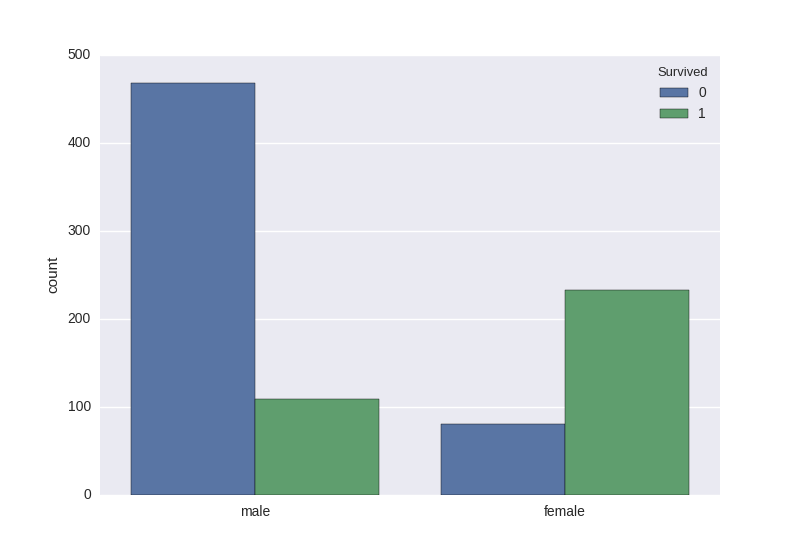
\includegraphics[width=0.49\textwidth]{sexSurv}
  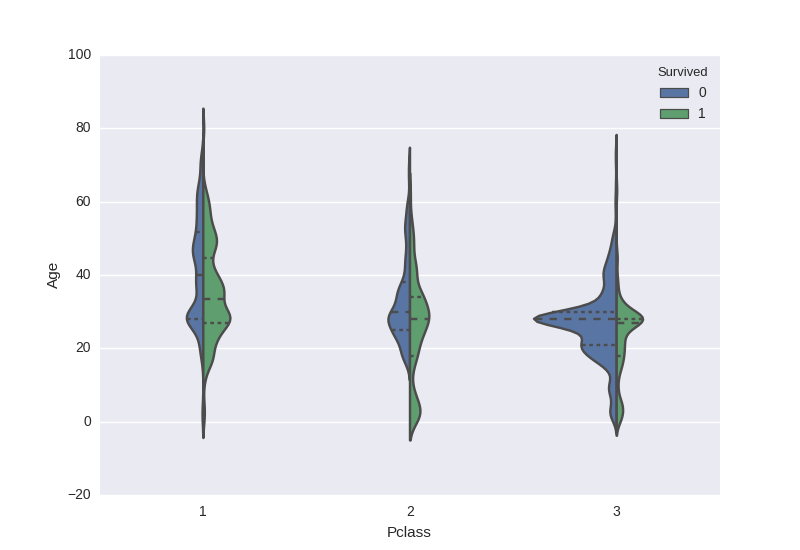
\includegraphics[width=0.49\textwidth]{classSurv}
  \caption{Left: Number of Titanic survivors depending on sex. Right: Violin graph for the fraction of survivors with age on the y axis and plotted for the three different passenger classes}
  \label{fig:titExpl}
\end{figure}

\subsection{Classification}
Looking at the score board and forums of this Kaggle competition, we see a few things: firstly, there are a lot of people with perfect 1.0 accuracy scores, and again a large number of submissions with 88\% accuracy.  Looking at the scripts these 88\%-submissions have, it is clear they all use the same genetic algorithm counting 48 lines of unreadable (and computer-generated) code.

On the forums it can be read that -- most likely -- the 1.0 scores were achieved by cheating, i.e., looking up the survival status of every person in the test set on the internet.  We also read that a score of 80\% can be seen as quite good, whereas above 84\% is almost unattainable.  Moreover, predicting survival on gender alone reaches 76\%; using a simple Random Forest model on a selected set of the features 77\%.  To score higher than this, more advanced models will have to be used.

In the previous exercise we practiced using different classifiers and models using cross-validation.  Therefore, the main point of this Kaggle competition is \emph{feature engineering}: combining, scrapping, adding, and otherwise transforming the available data to find features that are predictive of the final survival.  

Firstly we have to address the case of missing data.  The train set misses data on the Age, Cabin, and Embark columns; the test set on the Age, Cabin, and Fare columns.  The Embark and Fare columns contain only a very small number of missing values (2 and 1, resp.) which we can easily estimate.  The Cabin column is very hard to do anything with, so we opted to just drop this.  The Age column is the most interesting; Kaggle proposes to fill this with the median value,\footnote{Given the outlier distribution, median is possibly a better estimator than mean value.} either over the whole set or on a per-sex \& class basis.  We later estimated this Age using a simple Decision Tree regressor.

The Sex and Embarkation columns are enumerative; we can easily convert these to integers.  We will (initially) drop the columns Passenger ID, Name, Ticket, and Cabin, because they contain either useless or hard-to-parse data. As for transforming the data into usable features, the following ideas came up:
\begin{itemize}
	\item Create a \texttt{FamilySize} index, being \texttt{Parch + SibSp + 1}, and drop Parch and SibSp;
    \item Bin the Age column;
    \item Try to find families by using Cabin, Ticket, and Name information, together with FamilySize;
    \item Extract person titles from their Name.
\end{itemize}
This last item was frankly not ours; many Kaggle submissions use this feature with good results.  The reasoning behind the first idea is that parent-child or sibling-spouse relations really don't differ much; their separation could confuse the classifier.  The second item came from the class slides. As for idea three, although a genuinely very interesting problem, we chose not to pursue it, as it was infeasible in this time frame.

To test our models and features, we will take the train data set and divide it into three parts, train on the first two and generate a score on the third.  This gives us a crude estimate of the Kaggle score we might expect, and allows us to select between different models.  After model selection, we train on the entire data set and predict the survival of the remaining test subjects.  

This estimated accuracy is indeed very crude: see Table~\ref{tbl:results}.  In column (1), we used the features Age, Pclass, FamilySize, Sex, and Fare.  In column (2), we added to this a feature Title.  In column (3), we swapped Age for AgeBinned, with bins $[5, 15, 30, 45]$. The fourth experiment is based on (2), with Age predicted using a Decision Tree Regressor trained on Pclass, Sex, Fare, and Title.  

We immediately see a few things.  Firstly, the normally pretty good SVM classifier is constistently outperformed by the ensemble methods (which is why we didn't include them in later tests).   Secondly, the Kaggle score is consistently much lower than our estimated one. In column (2), we see that even though our AdaBoost algorithm was expected to win, the random forest classifier performed quite a lot better.  Thirdly, we see that our second idea of binning the ages has disastrous effects on the performance, even though it was expected to work well.  Lastly, we see that estimating the age using a regressor is predicted to work much better, but in actuality performs worse than just using a median value.

\begin{table}[h]
\centering
\begin{tabular}{lllll}
                      & (1)                       & (2)                       & (3)                      & (4) \\\toprule
Random Forest         & \textbf{81.1\%} (77.5\%)  & 80.8\% (78.9\%)           & 82.2\%                   & \textbf{84.5\%} (77.0\%) \\
Gradient Boosting     & 80.4\%                    & 80.8\%                    & \textbf{82.5\%} (76.6\%) & n.a. \\
AdaBoost              & 78.8\%                    & \textbf{82.2\%} (77.0\%)  & 81.8\% & 82.3\% \\
Decision Tree         & 75.6\%                    & 75.8\%                    & n.a. & n.a.\\
Linear SVM            & 78.1\%                    & 78.8\%                    & n.a. & n.a.\\
SVM with RBF kernel   & 79.8\%                    & 80.5\%                    & n.a. & n.a.\\\bottomrule
\end{tabular}
\vspace{2em}
\caption{Estimated and true Kaggle score for a variety of feature-classifier combinations.  Each classifier has its parameters tuned by means of a grid search using 5-fold cross-validation; each estimated result was found by training on two-thirds of the available data and testing on the rest.}
\label{tbl:results}
\end{table}

\subsubsection{Discussion and future work}
We look back on this Kaggle competition with mixed feelings.  We didn't do bad, with a 18/37 position (at 9:50 PM on Sunday).  But we expected a little more, more so because we already matched our best score of 78.9\% in one of our first submissions, not doing any classifier comparisons, model selections, or adding features.  This feeling is amplified by the fact that other submissions with comparable features and models yield accuracies in the 80.5\%-range.  All in all, we are quite happy with the tool we made and the analyses we did, but the score does not reflect our efforts.

Had we had more time, we would've loved to look more into our third idea above; extracting families from the data is (up to some extent) possible.  We can even verify our findings using the Parch and SibSp columns (and possibly the use of the internet).

\section{Research and Theory}

\subsection{State of the art solutions}
The ``Galaxy Zoo" data mining competition on Kaggle \cite{kaggle:galaxy} was set up to identify images of galaxies mad by the Sloan Digital Sky Survey \cite{sdss} and Hubbles CANDELS \cite{candels} by their shape. Previously the classification of these images was done in a crowd sourcing project where hundreds of volunteers classified galaxies using a search tree of questions. In fact the actual goal of the challenge is to predict the outcome of such a classification by the crowd and therefore it is a regression problem rather than a classification problem.

The competition ended on April 4th and the prize money went to the top three competitors. All three of them used a similar approach with a Convolutional Neural Network (CNN) and similar preprocessing. The Root Mean Square Error (RMSE) of the test set prediction was used as leaderbord score; the winner ended with a RMSE of $0.07467$. 

The concept of CNN is inspired by the visual cortex of animals, where the neurons all have a receptive field that overlaps with other the receptive fields of other neurons.  What a CNN does is to Machine Learn the appropriate filter to extract features from a certain type of data. This in contrast with extracting image features with a certain predefined filter. Because of the nature of the images in this data set, regular features used in computer vision would've returned bad results because they are generally accustomed to objects as we find them on earth. 

After the maximizing the number of found features, the filter can be applied to the images to extract the features and recognize certain structures of galaxies. 

\subsection{Measuring Numerical Error}
Classification algorithms predict a mapping from a set of attributes to a corresponding discrete value or label. It is easy to evaluate their performance: we simply check whether the predicted label was correct or not. A prediction is simply false or true. Regression algorithms predict numerical or continuous values: there is a continuous spectrum of errors, so we need a different measure of performance. Here we will discuss two such error measures: mean squared error (MSE) and mean absolute error (MAE). If $p_1, \dots, p_n$ are the predicted values and $a_1, \dots, a_n$ the actual values, then \cite{witten}:

\noindent\begin{minipage}{.5\linewidth}
\begin{equation*}
  \text{MSE} = \frac{1}{n} \sum_{i=1}^n (p_i - a_i)^2
\end{equation*}
\end{minipage}%
\begin{minipage}{.5\linewidth}
\begin{equation*}
  \text{MAE} = \frac{1}{n} \sum_{i=1}^n |p_i - a_i|
\end{equation*}
\end{minipage}

The model with the lowest MSE or MAE will then be the best performing model, i.e. the model with the best predictions. The main difference between MSE and MAE is the square in the MSE: the mean-squared error exaggerates the effect of outliers in the data. MAE does not have this effect, there all error sizes are treated equally. \cite{witten} Using MAE is recommended if many outliers are expected when evaluating the numerical performance of regression algorithms. Otherwise there is no difference for model evaluation.

There are also situations where the MSE and MAE are exactly the same. This happens when the terms in the summation are the same: $(p_i - a_i)^2 = |p_i - a_i| \implies p_i = a_i \lor p_i = a_i - 1$ for all $i$. For example, if $\vec{a}=(1, 2, 3)^T$ and $\vec{p}=(1, 1, 4)^T$, then MSE = MAE $= 2/3$. 

\iffalse
TODO: afmaken!!
Finally, let's look 
\fi

\subsection{Analysis of a less obvious data set}
We are given a set consisting of English text messages, each text labeled as either `spam' or `ham', with the latter signifying a bona fide SMS. 

Text mining is a very active area of both research and business.  Our specific task within text mining is akin to \emph{sentiment estimation}, and multiple Kaggle competitions have been done with this exact task in mind.  Most submissions seem to use a so-called \emph{bag-of-words} approach; instead of trying to parse the natural language contained in each text message, we create a `vocabulary' or dictionary of every word contained in this set of texts.\footnote{A few things are important here: firstly, the definition of a \emph{word}. Most often (as is in our case), a sequence of two or more alphanumeric characters surrounded by non-alphanumeric characters is deemed a word.  Moreover, these words need to be tokenized, which means given an index.  Often times people choose to convert every word to lowercase, but other transformations are also possible.}
The resulting histograms (defined as the number of each word a text contains) then become our feature vectors.  As we did before, we subdivide the data set into a training and test set, retaining one third of the total size for testing.\footnote{In order to reduce noise, we repeat each experiment 10 times, and average the result.}

In practice, using these histograms as-is yields some inconsistencies: consider a text message $S$, with some distribution $D$. Then the message $SSSS$ (four repetitions of $S$) has distribution $4D$, which is very different from $D$, although the two messages discuss the same topic and will hence carry the same label.  To counter this, well-performant Kaggle submissions will often divide these histograms by their sum, yielding something like a ``frequency histrogram''.

A large variety of classifiers can be used on tasks like these.  Looking at the sklearn flow chart,\cite{sklearnflow} we see that the SVM with a linear kernel, Stochastic GD classifier, and Naive Bayes are good contenders.  Again, these all have their respective parameters which we can optimize using a grid search and cross-validation.

Running the above method in its most simple form yields 8713 features per sample, with results visible in the column (1) of Table~\ref{tbl:sms}.  The other columns show results after distillation of the features: (2) we have 4213 features left if we remove all words that occur in only one text message; (3) 3965 features result after removing \emph{stop words} (e.g., `a', `the', `which') from the texts before tokenizing.

\begin{wraptable}{r}{0.4\linewidth}
\vspace{-2em}
\centering
\begin{tabular}{lccc}
& (1) & (2) & (3) \\\toprule
\# features & 8713 & 4213 & 3965 \\ \midrule
DecisionTree 	& 96.5\% & 96.3\% & 96.1\%\\
Linear SVM 		& 98.2\% & 98.4\% & 98.0\%\\
Stochastic GD 	& 98.2\% & 98.4\% & 98.2\%\\
Multinomial NB 	& 97.2\% & 98.1\% & 98.2\%\\\bottomrule
\end{tabular}
\caption{Accuracy on a held-out test set for different classifiers, for different feature settings.  All classifiers have their parameters optimized by cross-validation, and each accuracy is found by averaging over 10 experiments.}
\label{tbl:sms}
\end{wraptable}

Looking at this table, we see that removing single-document words makes hardly any difference in terms of accuracy, and that removing the stop words doesn't do much either.  As far as model selection goes, we see that the linear SVM and Stochastic Gradient Descent classifiers perform best, with comparable results.  This is again in accordance with the previously mentioned flow chart.

If we think about how the linear SVM works, we can infer some interesting points from the weights.\cite{stackoverflow}  Large absolute values have a big say in the final class prediction; negative weights correspond to the negative class (in our case ham) and vice versa. Using the linear SVM-model that yielded the best results, we can come up with two lists of the `hammiest' and `spammiest words', which are pretty much in line with what one would expect.
\begin{description}
\item[Hammiest words] liked, happy, mail, yup, ok, morning, cool, cancer
\item[Spammiest words] uk, www, claim, service, filthy, win, games
\end{description}

\bibliography{references}
\bibliographystyle{unsrt}

\end{document}
